\subsection{Estudo do espaço de trabalho do manipulador}

Para uma avaliação técnica das soluções é necessária a análise do espaço de
trabalho, assim como a manutenção de sua manipulabilidade em toda a trajetória a
ser traçada. A escolha de um manipulador industrial, no contexto da aplicação
desejada, é um compromisso entre o tamanho do manipulador e o espaço disponível.
Um manipulador de grande porte garante que todos os pontos a serem metalizados
sejam processados sem problemas, entretanto pode tornar inviável que o mesmo se
movimente no espaço confinado e consiga passar pelos acessos limitados. Por esse
motivo, é necessário que a escolha do manipulador seja ótima no aspecto do
tamanho do manipulador e de seus graus de liberdade, para que seja possível de
se especificar o menor manipulador possível que atenda com uma certa margem de
segurança a tarefa a ser realizada.

A análise do espaço de trabalho do manipulador será realizada utilizando-se
ferramentas de simulação 3D específicas para manipuladores robóticos. No
processo de estudo de viabilidade técnica serão utilizados dois
\textit{frameworks:} \textit{OpenRAVE - Open Robotics Automation Virtual
Environment}, utilizado para uma análise detalhada do espaço de trabalho do
robô e o \textit{MoveIt!}, utilizado principalmente para o planejamento e
análise de trajetórias e controle de manipuladores.

A primeira etapa no estudo consiste na importação dos modelos desenvolvidos em
\textit{SolidWorks} para o ambiente de simulação do \textit{OpenRAVE}. O Aro
câmara e o rotor tem papel fundamental na descrição do espaço disponível para a
realização do processo de metalização. A figura \ref{fig::rotor_openrave}
ilustra o aro câmara e o rotor no ambiente de simulação do \textit{OpenRAVE}. 

\begin{figure}[h!]
\centering
	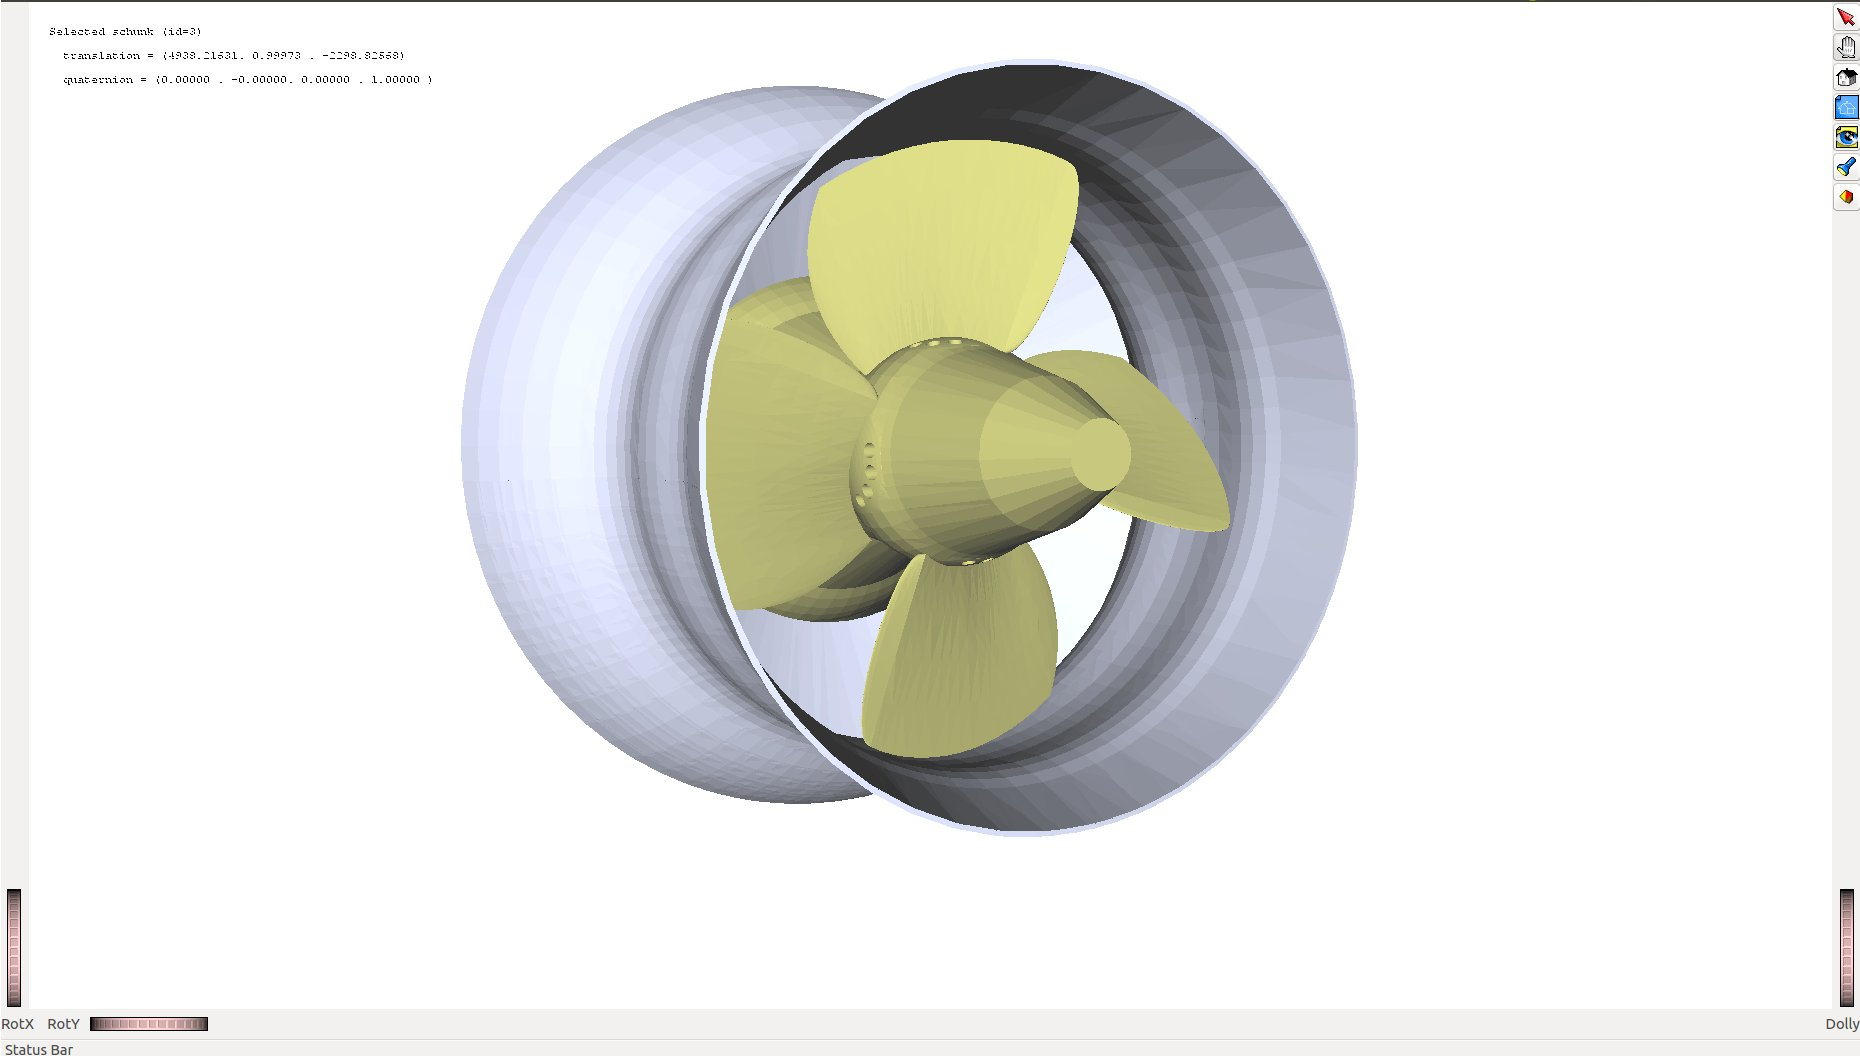
\includegraphics[width=\columnwidth]{figs/openrave/rotor_openrave}
	\caption{Turbina simulada no ambiente do \textit{OpenRAVE}.}
	\label{fig::rotor_openrave}
\end{figure}

Cada manipulador robótico a ser simulado deve ter sua estrutura modelada e suas
juntas assinaladas. Cada elo do robô deve ser modelado ou importado de um
arquivo externo e sua posição referente ao eixo de coordendas da base do
manipulador, assim como o eixo de rotação e os ângulos
limites de cada junta devem ser descrito de maneira a formar uma representação
completa do manipulador no ambiente de simulação. Para uma primeira análise,
foram escolhidos dois manipuladores industriais padrão com dimensões dentro de
faixas que representassem um manipulador de médio e grande porte. Como
manipulador de médio porte foi escolhido o modelo \textit{KR 30} do fabricante
\textit{Kuka Robotics} e para o manipulador de grande porte o modelo
\textit{KR 30l16}, do mesmo fabricante, foi selecionado.
A escolha desses manipuladores é justificada, em um primeiro momento, para uma
familiarização com o ambiente de simulação e uma perspectiva das dimensões
necessárias e limites para manipuladores industriais. 

O manipulador \textit{Kr30} é um manipulador de médio porte, com capacidade de
30kg de carga, 45kg de carga adicional, alcance máximo de 2033mm. A figura
\ref{fig::kukakr30_openrave} ilustra o modelo gerado no ambiente de simulação. 

\begin{figure}[h!]
\centering
	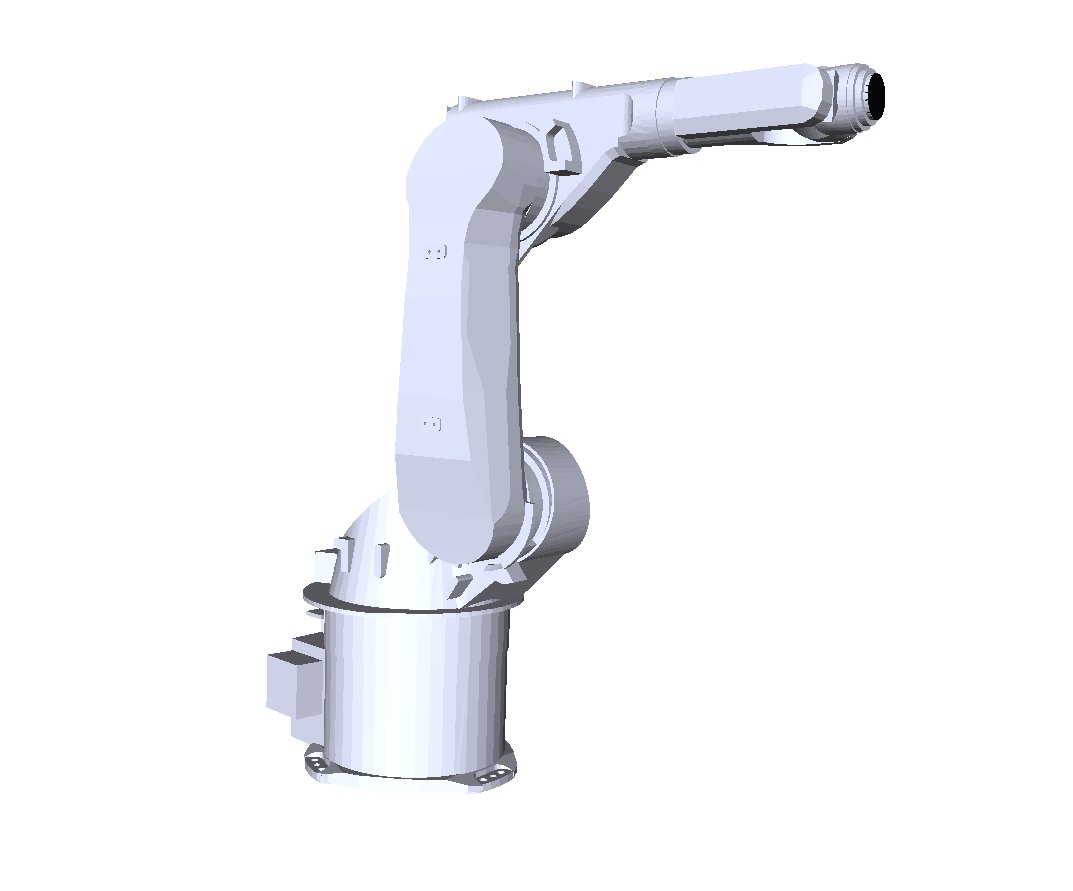
\includegraphics[width=0.8\columnwidth]{figs/openrave/kukakr30_openrave}
	\caption{Manipulador industrial modelo Kuka-KR30 no ambiente de simulação.}
	\label{fig::kukakr30_openrave}
\end{figure}

Por sua vez, o manipulador de grande porte, ilustrado na figura
\ref{fig::kukakr30l16_openrave} é uma versão extendida do manipulador \textit{KR
30} com alcande de 3102mm e carga reduzida para 16kg no efetuador e 45kg de carga adicional. Mesmo com a redução de carga o manipulador ainda se
encontra dentro de uma região aceitável, visto que o peso do sistema de
metalização é de 8,5kg.

\begin{figure}[h!]
\centering
	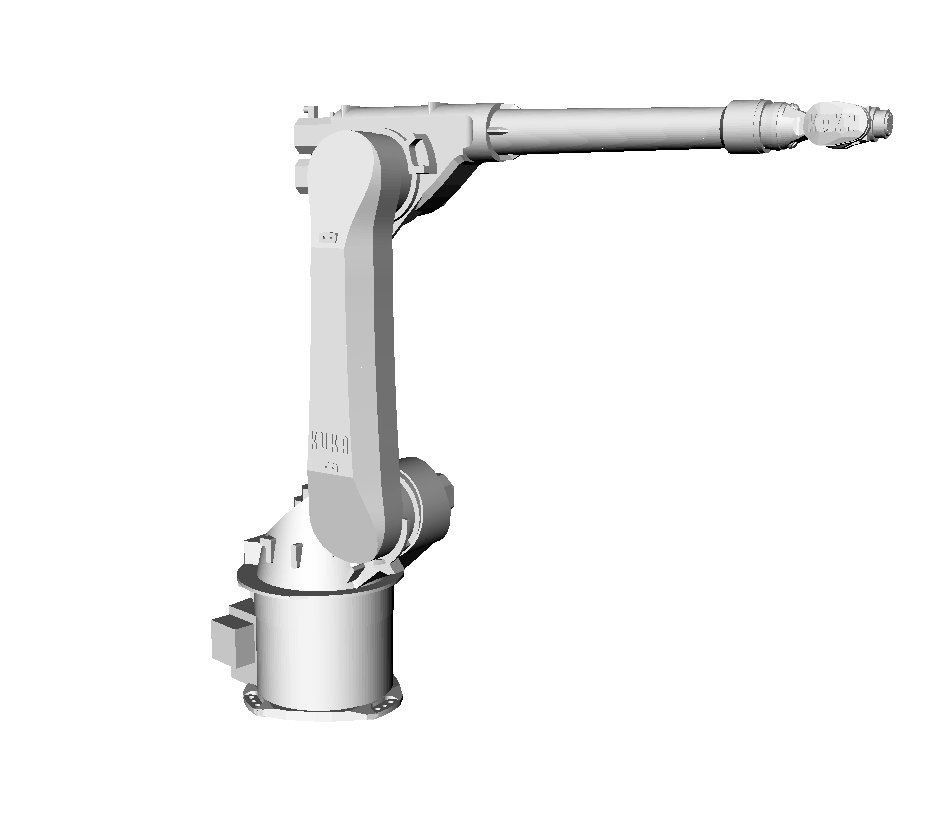
\includegraphics[width=0.8\columnwidth]{figs/openrave/kukakr30l16_openrave}
	\caption{Manipulador industrial modelo Kuka-KR30l16 no ambiente de simulação.}
	\label{fig::kukakr30l16_openrave}
\end{figure}
